% --- Pipeline parallelism and 3D parallelism ---
\begin{frame}{Naive Model Parallelism Wastes Almost Everything}
  \begin{itemize}\footnotesize\itemsep0.25em
    \item[\textcolor{red}{$\blacktriangleright$}] The obvious way to fit a deep model on $p$ devices is to give each device a contiguous slice of the layers. It works, and it is catastrophically slow.
    \item[\textcolor{red}{$\blacktriangleright$}] Layer $i+1$ cannot start until layer $i$ finishes, so at any instant \textbf{exactly one} device is doing work and $p-1$ are idle. Utilisation is $1/p$.
  \end{itemize}
  \vspace{0.2em}
  \centering
  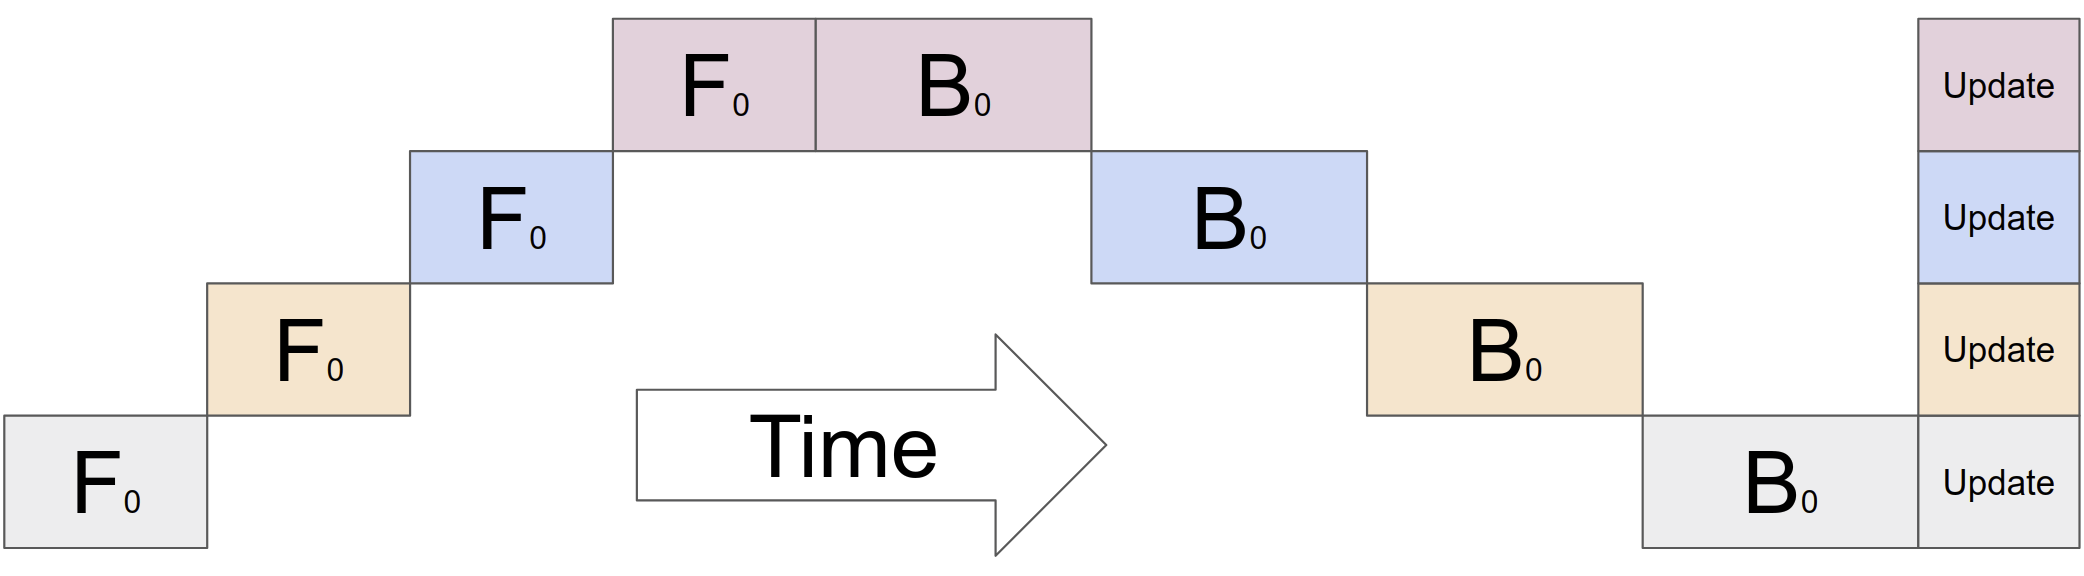
\includegraphics[width=0.9\textwidth,height=0.36\textheight,keepaspectratio]{images/distributed-training/gpipe_fig2b_naive_model_parallelism.png}\\[0.25em]
  {\scriptsize Naive model parallelism across four accelerators: one mini-batch $F_0$ walks up the stack and back down, and the rest of the cluster waits. Huang et al., ``GPipe: Efficient Training of Giant Neural Networks using Pipeline Parallelism,'' \href{https://arxiv.org/abs/1811.06965v5}{arXiv:1811.06965v5}, Figure 2(b).}
  \vspace{0.3em}
  \begin{itemize}\footnotesize
    \item[\textcolor{red}{$\blacktriangleright$}] The fix is the same one that made CPU pipelines work: keep several items in flight so the stages overlap.
  \end{itemize}
\end{frame}

\begin{frame}{GPipe: Micro-batching Fills the Pipe}
  \centering
  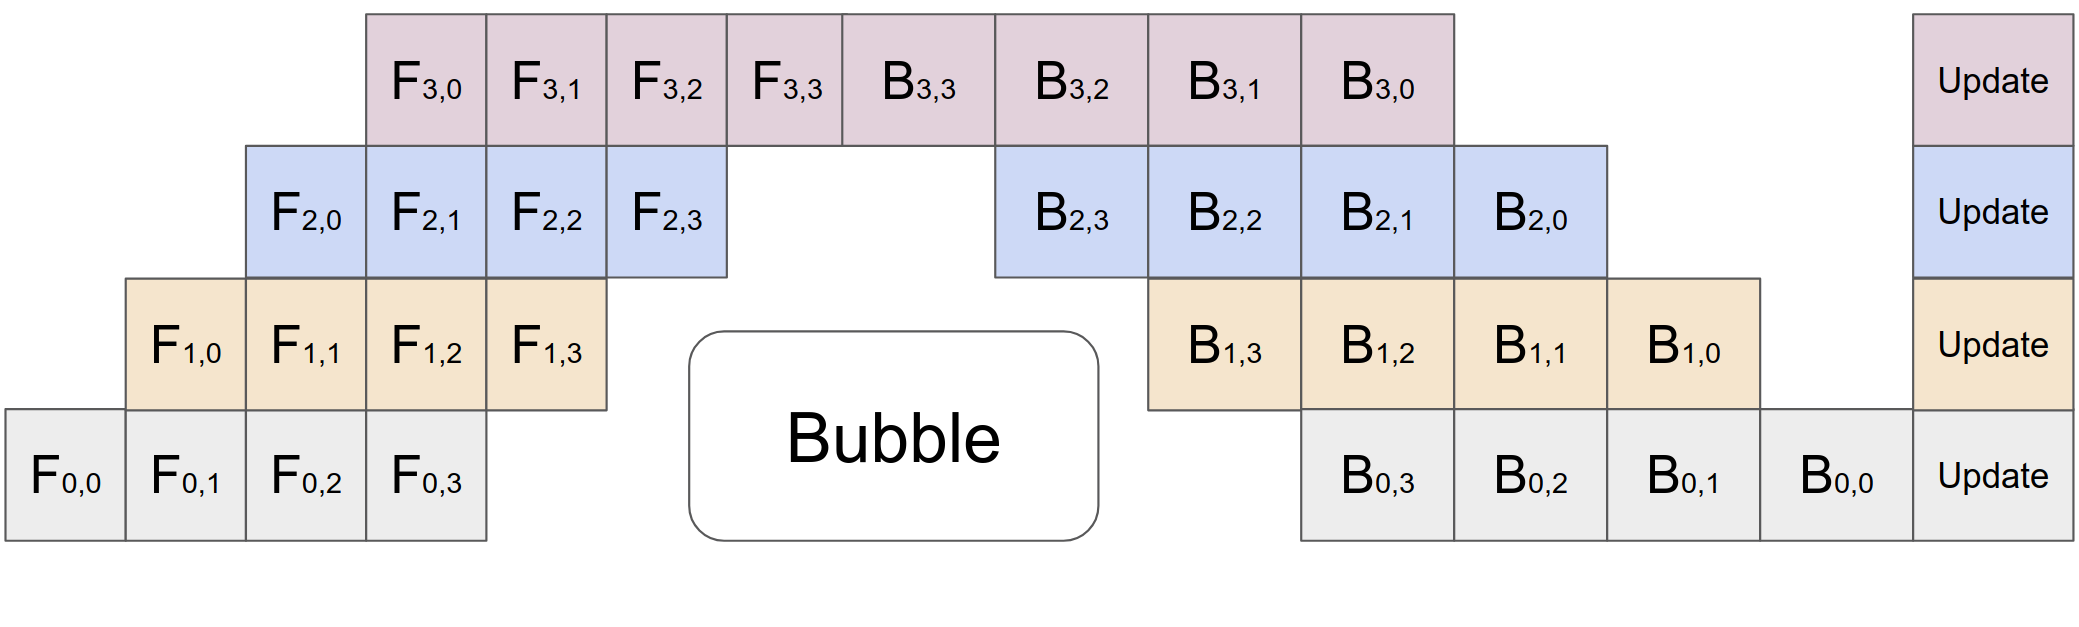
\includegraphics[width=0.9\textwidth,height=0.34\textheight,keepaspectratio]{images/distributed-training/gpipe_fig2c_pipeline_parallelism.png}\\[0.25em]
  {\scriptsize The same four devices after the mini-batch is split into four micro-batches. Huang et al., \href{https://arxiv.org/abs/1811.06965v5}{arXiv:1811.06965v5}, Figure 2(c).}
  \vspace{0.4em}
  \begin{itemize}\footnotesize\itemsep0.25em
    \item[\textcolor{red}{$\blacktriangleright$}] Split the mini-batch into $m$ \textbf{micro-batches} and feed them in sequence. While device 1 works on micro-batch 2, device 2 works on micro-batch 1, and so on. Gradients are accumulated and applied once, at the end --- so the optimizer semantics are \emph{identical} to single-device training.
    \item[\textcolor{red}{$\blacktriangleright$}] The idle wedges at the start and end are the \textbf{pipeline bubble}: $p-1$ forward passes waiting for the pipe to fill, and $p-1$ backward passes waiting for it to drain.
    \item[\textcolor{red}{$\blacktriangleright$}] Communication is \textbf{point-to-point}, not a collective: each stage sends one activation tensor of size $b \cdot s \cdot h$ to its successor. This is why pipeline parallelism tolerates slow inter-node links --- it is the cheapest axis to stretch across a network.
  \end{itemize}
\end{frame}

\begin{frame}[allowframebreaks]{The Bubble, Quantified}
  \begin{itemize}\itemsep0.35em
    \item[\textcolor{red}{$\blacktriangleright$}] Write $p$ for the number of pipeline stages, $m$ for the number of micro-batches, and $t_f, t_b$ for one micro-batch's forward and backward time. The bubble is $p-1$ forward passes plus $p-1$ backward passes:
      \[
        t_{pb} = (p-1)(t_f + t_b), \qquad t_{id} = m\,(t_f + t_b),
        \qquad \frac{t_{pb}}{t_{id}} = \boxed{\frac{p-1}{m}}.
      \]
    \item[\textcolor{red}{$\blacktriangleright$}] GPipe's own paper states the same quantity as a fraction of \emph{total} time, $\dfrac{p-1}{m+p-1}$, and reports the overhead ``negligible when $m \geq 4p$''. The two expressions are the same number with different denominators; quote whichever your audience expects.
    \item[\textcolor{red}{$\blacktriangleright$}] \textbf{Worked example.} $p = 8$ stages, $m = 64$ micro-batches: bubble $= 7/64 \approx 11\%$ of ideal time. Halve the micro-batches to $m = 32$ and it doubles to $22\%$.
    \item[\textcolor{red}{$\blacktriangleright$}] So you want $m \gg p$ --- and that is exactly where GPipe's memory problem appears. The all-forward-then-all-backward schedule keeps activations for \textbf{all $m$ micro-batches} alive at once, so shrinking the bubble inflates the activation memory linearly.
    \item[\textcolor{red}{$\blacktriangleright$}] Two constraints pulling in opposite directions through the same variable. Resolving that tension is what the next schedule does.
  \end{itemize}
  \vspace{0.1em}
  {\scriptsize Narayanan et al., \href{https://arxiv.org/abs/2104.04473v5}{arXiv:2104.04473v5}, Section 2.2.1; Huang et al., \href{https://arxiv.org/abs/1811.06965v5}{arXiv:1811.06965v5}, Section 2.}
\end{frame}

\begin{frame}{1F1B: Same Bubble, Bounded Memory}
  \centering
  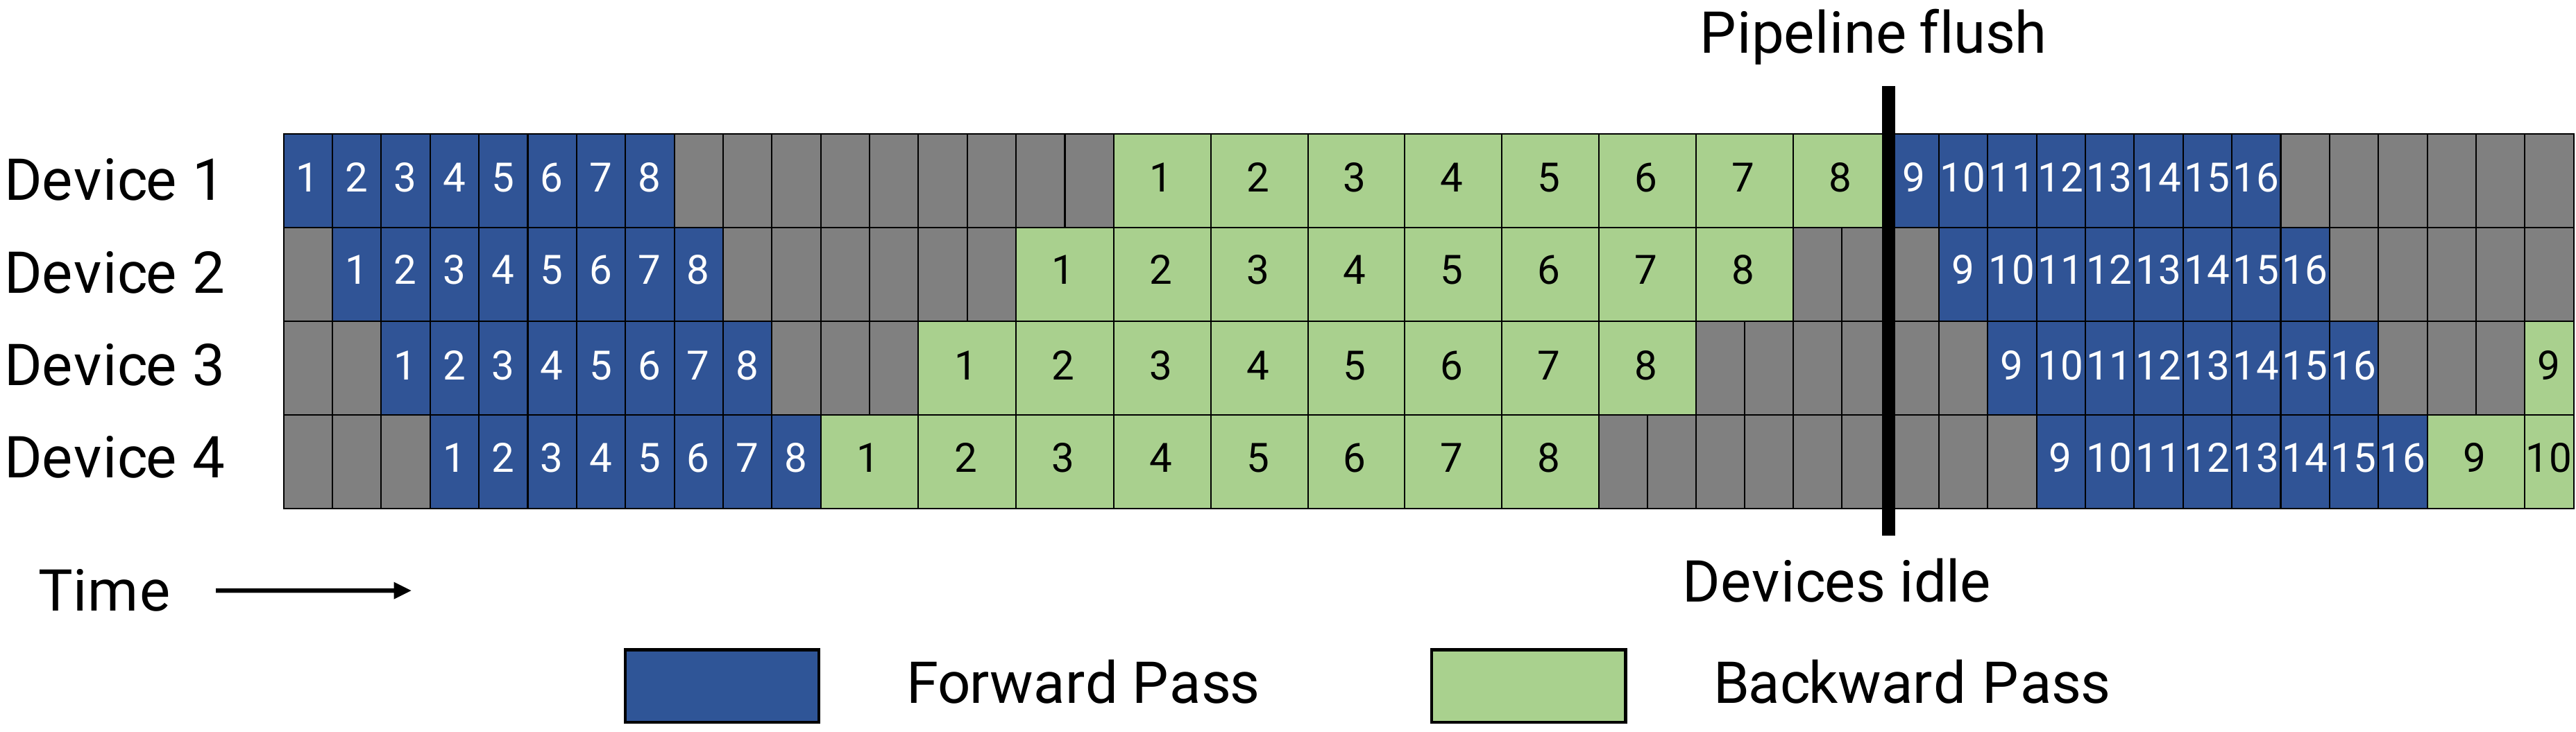
\includegraphics[width=0.94\textwidth,height=0.33\textheight,keepaspectratio]{images/distributed-training/megatron3d_fig3_gpipe_schedule_bubble.png}\\[0.2em]
  {\scriptsize The GPipe schedule: all forwards (blue), then all backwards (green), then a flush. Grey is bubble. Narayanan et al., \href{https://arxiv.org/abs/2104.04473v5}{arXiv:2104.04473v5}, Figure 3.}
  \vspace{0.4em}
  \begin{itemize}\footnotesize\itemsep0.25em
    \item[\textcolor{red}{$\blacktriangleright$}] \textbf{PipeDream-Flush (1F1B)} keeps the identical bubble but reorders the work: after a short warm-up, every device alternates \emph{one forward, one backward}.
    \item[\textcolor{red}{$\blacktriangleright$}] Because a micro-batch's backward pass now runs almost immediately after its forward pass, the number of micro-batches whose activations must be stashed drops from $m$ to \textbf{at most $p$}.
    \item[\textcolor{red}{$\blacktriangleright$}] When $m \gg p$ --- exactly the regime you want for a small bubble --- this is a large memory saving for free. 1F1B is the default schedule in Megatron-LM, DeepSpeed, and PyTorch's pipelining API.
    \item[\textcolor{red}{$\blacktriangleright$}] The stages are also unequal in memory: stage 0 holds the most in-flight activations, stage $p-1$ the fewest. Balanced \emph{layer} assignment does not give balanced \emph{memory}.
  \end{itemize}
\end{frame}

\begin{frame}{Interleaving: Buying the Bubble Down With Communication}
  \centering
  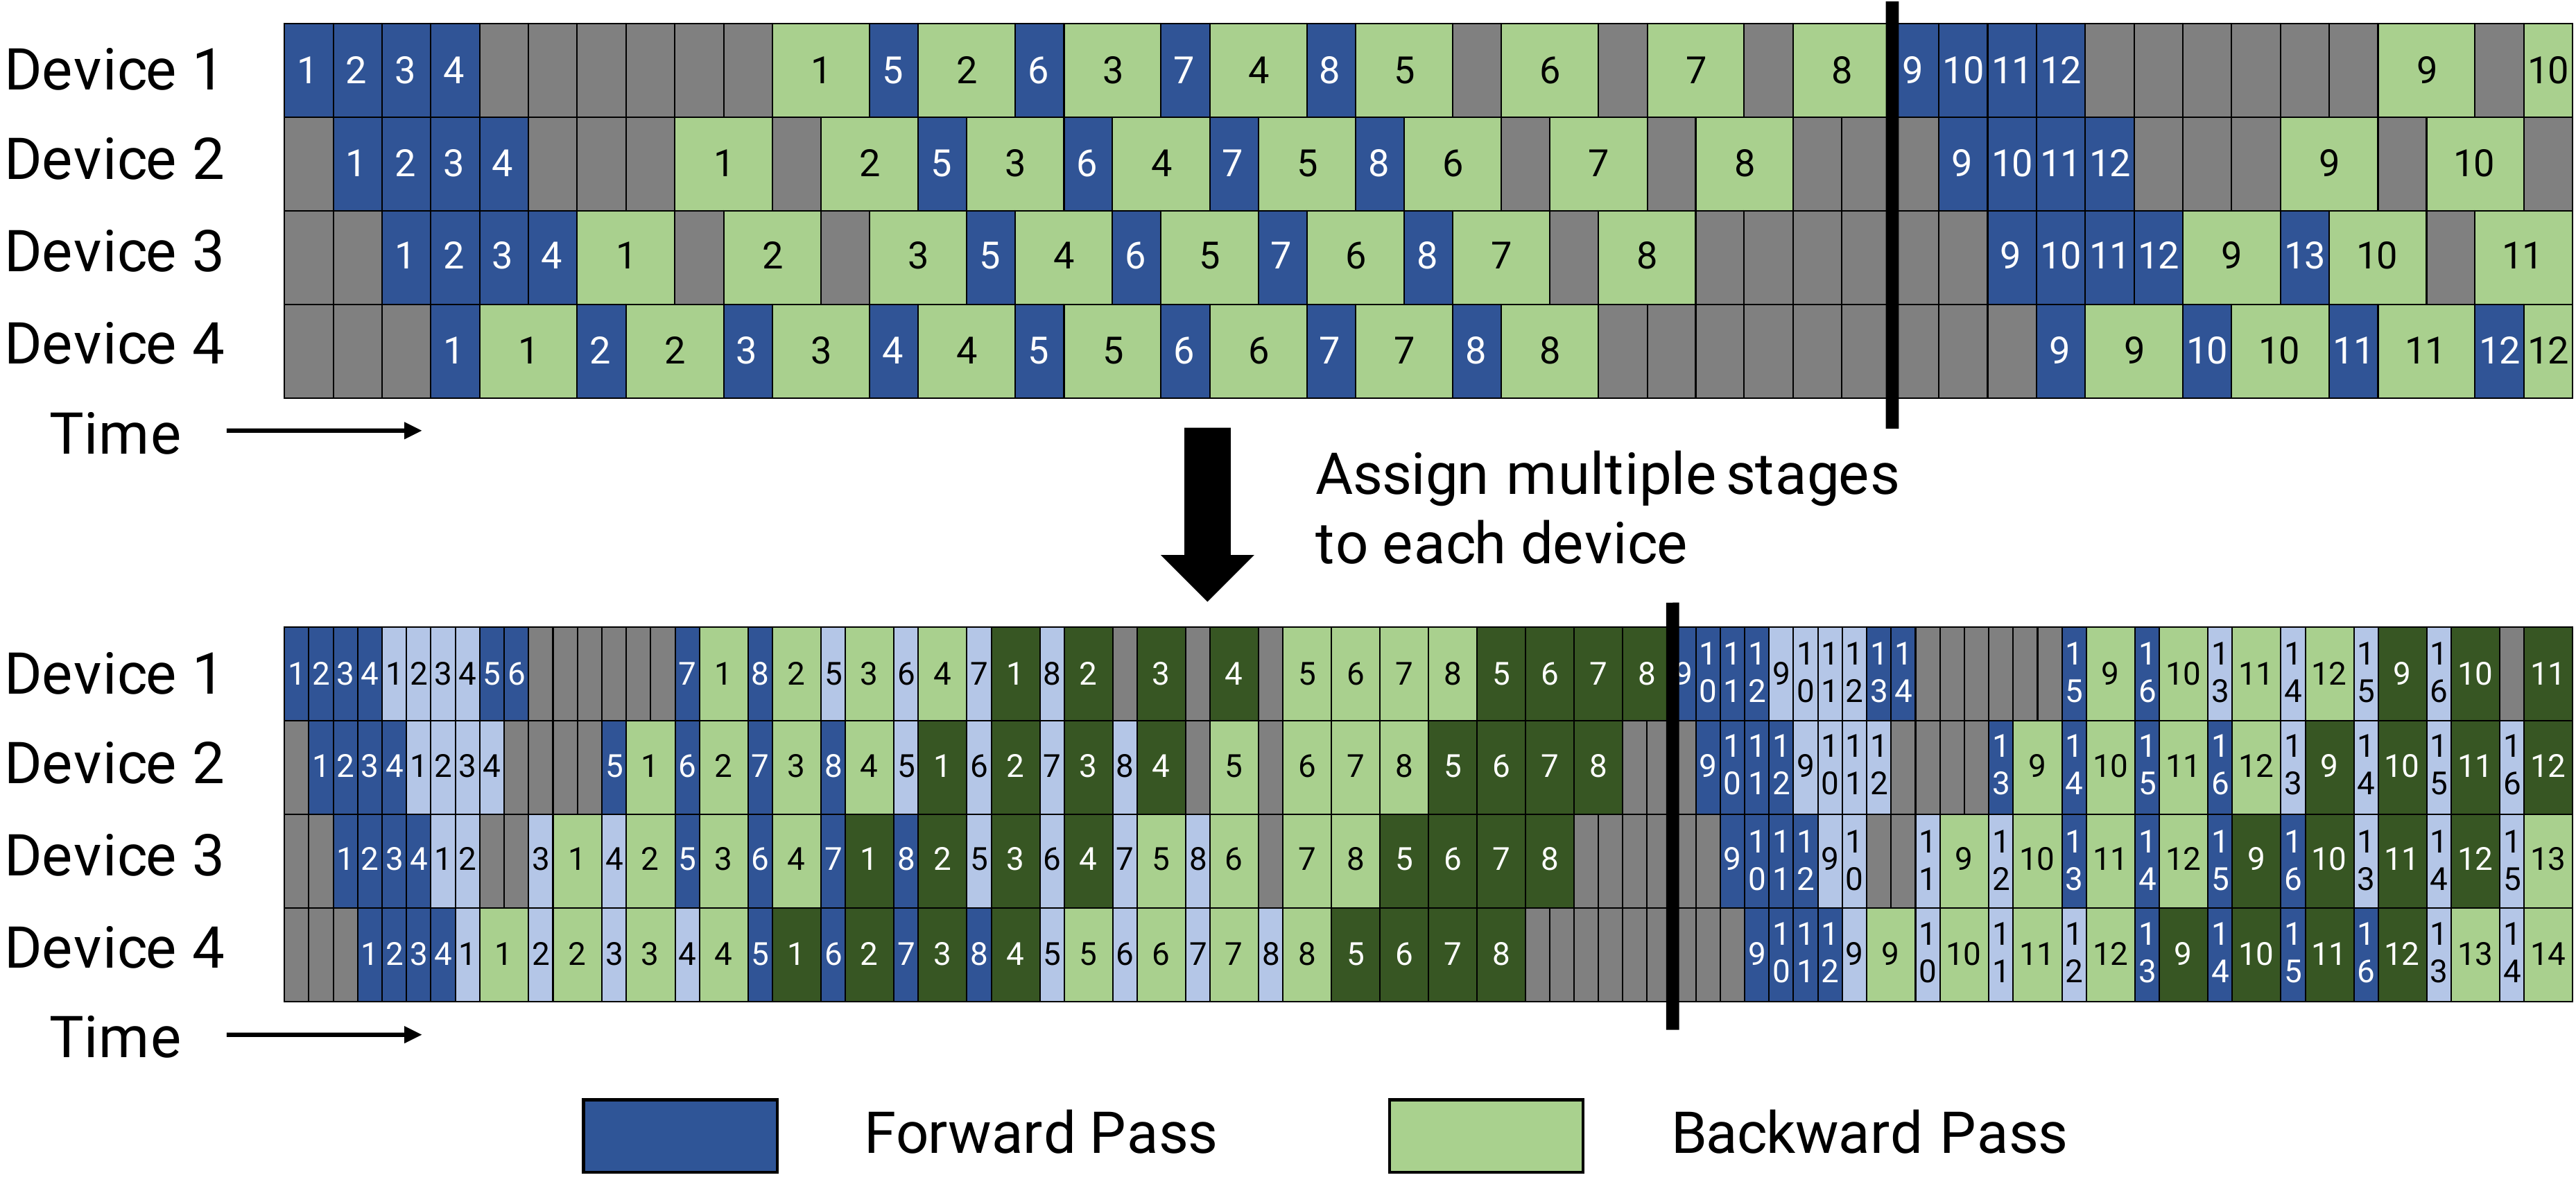
\includegraphics[width=0.9\textwidth,height=0.36\textheight,keepaspectratio]{images/distributed-training/megatron3d_fig4_default_and_interleaved_1f1b.png}\\[0.2em]
  {\scriptsize Top: default 1F1B. Bottom: interleaved 1F1B with $v = 2$ chunks per device; the flush happens sooner. Narayanan et al., \href{https://arxiv.org/abs/2104.04473v5}{arXiv:2104.04473v5}, Figure 4.}
  \vspace{0.35em}
  \begin{itemize}\footnotesize\itemsep0.2em
    \item[\textcolor{red}{$\blacktriangleright$}] Give each device $v$ non-contiguous \textbf{model chunks} instead of one contiguous block (device 1 gets layers $1,2$ and $9,10$; device 2 gets $3,4$ and $11,12$; and so on). Each chunk is smaller, so $t_f$ and $t_b$ shrink by $v$ and the bubble becomes $\dfrac{1}{v}\cdot\dfrac{p-1}{m}$.
    \item[\textcolor{red}{$\blacktriangleright$}] It is not free: the point-to-point communication volume also increases by $v$. Interleaving therefore pays off precisely when the pipeline links are fast enough to absorb it --- which is why Megatron pairs it with the scatter/gather optimisation over a node's multiple InfiniBand cards.
    \item[\textcolor{red}{$\blacktriangleright$}] Requires $m$ to be an integer multiple of $p$. Reported gain: over \textbf{10\%} throughput at comparable memory.
  \end{itemize}
\end{frame}

\begin{frame}{3D Parallelism: Using All Three Axes at Once}
  \begin{columns}[T,onlytextwidth]
    \column{0.5\textwidth}
      \centering
      \vspace{0.6em}
      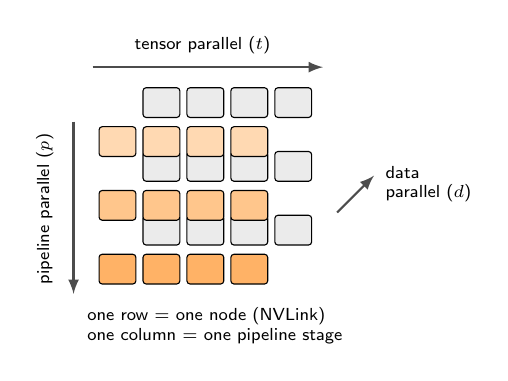
\begin{tikzpicture}[font=\sffamily\scriptsize, >=latex, scale=0.9,
          every node/.style={transform shape},
          g/.style={draw, minimum width=0.52cm, minimum height=0.42cm, rounded corners=0.04cm}]
        % Back data-parallel replica (drawn first so the front overlaps it)
        \foreach \pp in {0,1,2} {
          \foreach \tp in {0,1,2,3} {
            \node[g, fill=black!8] at ({0.62*\tp+0.62},{-0.9*\pp+0.55}) {};
          }
        }
        % Front data-parallel replica
        \foreach \pp/\col in {0/orange!30, 1/orange!45, 2/orange!60} {
          \foreach \tp in {0,1,2,3} {
            \node[g, fill=\col] at ({0.62*\tp},{-0.9*\pp}) {};
          }
        }
        % Axis annotations, placed clear of both replicas.
        \draw[->, thick, black!70] (-0.35,1.05) -- (2.9,1.05);
        \node[anchor=south, font=\sffamily\scriptsize] at (1.2,1.12) {tensor parallel ($t$)};
        \draw[->, thick, black!70] (-0.62,0.28) -- (-0.62,-2.15);
        \node[rotate=90, anchor=south, font=\sffamily\scriptsize] at (-0.78,-0.95) {pipeline parallel ($p$)};
        \draw[->, thick, black!70] (3.1,-1.0) -- (3.62,-0.48);
        \node[anchor=west, font=\sffamily\scriptsize, align=left] at (3.66,-0.6) {data\\parallel ($d$)};
        \node[anchor=west, font=\sffamily\scriptsize, align=left] at (-0.55,-2.6)
          {one row $=$ one node (NVLink)\\one column $=$ one pipeline stage};
      \end{tikzpicture}
    \column{0.48\textwidth}
      \begin{itemize}\footnotesize\itemsep0.3em
        \item[\textcolor{red}{$\blacktriangleright$}] The three axes are orthogonal and multiply:
          $\text{GPUs} = t \times p \times d$.
        \item[\textcolor{red}{$\blacktriangleright$}] They are assigned to the hardware by \textbf{communication intensity}: tensor parallelism gets the fastest links (inside a node), pipeline parallelism the slowest (point-to-point across nodes), and data parallelism whatever is left, because DDP traffic can be overlapped.
        \item[\textcolor{red}{$\blacktriangleright$}] Sequence parallelism (next section) adds a fourth, and expert parallelism a fifth --- which is why practitioners now say ``4D'' or ``5D'' as often as ``3D''.
        \item[\textcolor{red}{$\blacktriangleright$}] \textbf{Mixture-of-Experts routing} is its own parallel axis (each expert lives on its own device, connected by an all-to-all). Deck 13 owns that treatment; here it is enough to know that expert parallelism composes with the three axes above.
      \end{itemize}
  \end{columns}
\end{frame}

\begin{frame}{A Worked Cluster Plan}
  \begin{itemize}\footnotesize\itemsep0.3em
    \item[\textcolor{red}{$\blacktriangleright$}] \textbf{Given:} 64 nodes, 8 H100 SXM (80\,GB) each, NVLink inside a node and InfiniBand between nodes. \textbf{Target:} pre-train a 175B-parameter model.
    \item[\textcolor{red}{$\blacktriangleright$}] \textbf{Step 1 --- tensor parallel.} Set $t = 8$: fill the node, never cross the network with an unhideable all-reduce.
    \item[\textcolor{red}{$\blacktriangleright$}] \textbf{Step 2 --- pipeline parallel.} Model states are $16\Psi = 2.8$\,TB. With $t = 8$ alone each GPU would still hold $350$\,GB. Choose $p = 8$, giving a model-parallel size $M = t \cdot p = 64$ and $2.8\,\text{TB}/64 = 43.8$\,GB of model states per GPU.
    \item[\textcolor{red}{$\blacktriangleright$}] \textbf{Step 3 --- data parallel.} $d = 512 / 64 = 8$ replicas. Layering a ZeRO-1 distributed optimizer across those 8 ranks shards the $12\Psi$ optimizer term once more:
      \[
        \frac{4\Psi}{M} + \frac{12\Psi}{M \cdot d} = \frac{700}{64} + \frac{2100}{512} = 10.9 + 4.1 = \mathbf{15.0\ GB\ per\ GPU},
      \]
      leaving roughly 65\,GB per GPU for activations, communication buffers, and headroom.
    \item[\textcolor{red}{$\blacktriangleright$}] \textbf{Step 4 --- micro-batches.} Pick $m = 64$ per data-parallel replica: bubble $= (p-1)/m = 7/64 \approx 11\%$, or $5.5\%$ with $v = 2$ interleaving. Global batch $= b \cdot m \cdot d$.
    \item[\textcolor{red}{$\blacktriangleright$}] \textbf{Sanity check against reality:} Narayanan et al.\ ran a \emph{1-trillion}-parameter model on 3072 A100s at \textbf{502 petaFLOP/s}, 52\% of theoretical peak, using exactly this recipe.
  \end{itemize}
\end{frame}

\begin{frame}[allowframebreaks]{Choosing the Configuration}
  \begin{itemize}\itemsep0.4em
    \item[\textcolor{red}{$\blacktriangleright$}] \textbf{Takeaway \#1:} use tensor parallelism up to the number of GPUs in a server, then pipeline parallelism across servers.
    \item[\textcolor{red}{$\blacktriangleright$}] \textbf{Takeaway \#2:} choose the model-parallel size $M = t \cdot p$ so that parameters and intermediate state fit in memory, then use data parallelism to consume the remaining GPUs.
    \item[\textcolor{red}{$\blacktriangleright$}] \textbf{Takeaway \#3:} the optimal micro-batch size $b$ depends on the model, the pipeline depth $p$, the data-parallel size $d$, and the global batch $B$ --- there is no universal value; measure it.
    \item[\textcolor{red}{$\blacktriangleright$}] Practical failure modes worth naming out loud:
      \begin{itemize}\itemsep0.2em\footnotesize
        \item \textbf{Unbalanced stages.} The embedding and output layers are much heavier than a transformer block, so an even layer split gives an uneven \emph{time} split, and the slowest stage sets the pace of the whole pipeline.
        \item \textbf{Too few micro-batches.} A large $p$ with a small global batch produces a bubble that dwarfs the savings.
        \item \textbf{Stragglers.} Every collective is a barrier; one slow GPU or one flapping network link slows all $t \cdot p \cdot d$ of them.
      \end{itemize}
    \item[\textcolor{red}{$\blacktriangleright$}] \textbf{Checkpointing at this scale} is itself a distributed problem: state must be saved from every rank, asynchronously, with enough metadata to restore under a \emph{different} parallel layout. PyTorch Distributed Checkpoint and Megatron's converters exist for exactly this.
  \end{itemize}
  \vspace{0.1em}
  {\scriptsize Takeaways quoted from Narayanan et al., \href{https://arxiv.org/abs/2104.04473v5}{arXiv:2104.04473v5}, Section 3.}
\end{frame}
